
\chapter{Results} 

\label{Chapter5}

%----------------------------------------------------------------------------------------

In this chapter we discuss the results obtained with our model. First, we analyze how the model works in a given (original) resolution, so that we can be confident about its performance. Then, we consider how the accuracy changes with the resolution and within the categories. Finally, we discuss the cost en environment impact around Satellite imagery to analyze the world. 

\section{Transfer Learning on Aerial Imagery}

\section{Man-made Structures Detection at Different Scale}

\begin{figure}[h!]
	\centering
	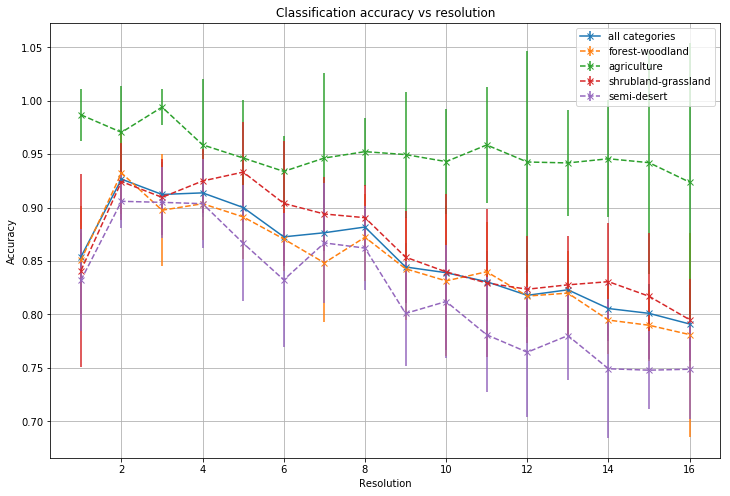
\includegraphics[width=\textwidth]{Figures/results/results_1m_all_categories.png}
	\captionsetup{width=1\linewidth}
	\caption{\textbf{$1m$ dataset}}
	\label{fig:acc_1m_all_cat}
\end{figure}

\begin{figure}[h!]
	\centering
	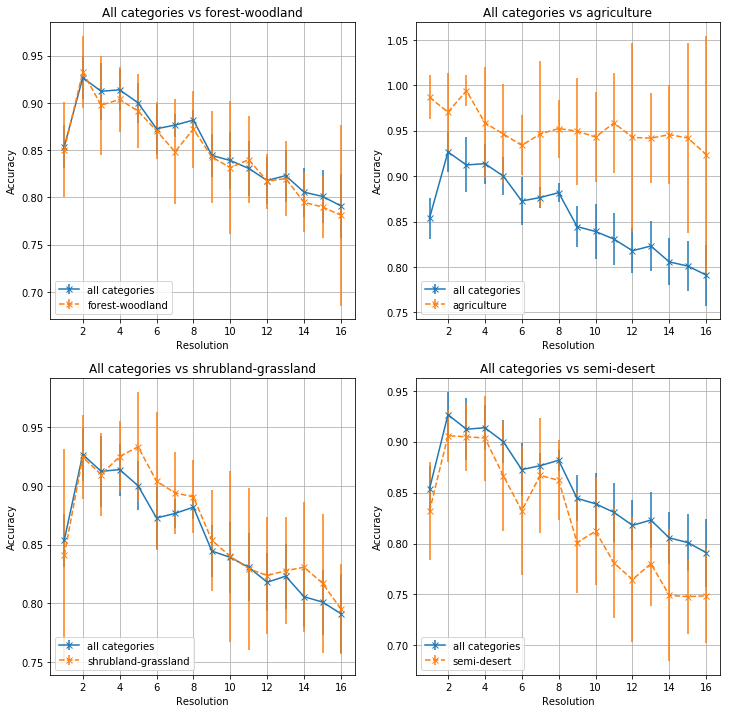
\includegraphics[width=\textwidth]{Figures/results/results_1m_by_category.png}
	\captionsetup{width=1\linewidth}
	\caption{\textbf{$1m$ dataset}}
	\label{fig:acc_1m_byl_cat}
\end{figure}



\section{Cost and Environment impact}
